\section{Critical Analysis and Limitations}
\label{sec:critical-analysis}

\subsection{Per-Category Weaknesses}
\label{sec:critical-analysis:per-category}

This subsection revisits each of the five taxonomy axes from
Section~\ref{sec:taxonomy} in turn, this time asking not how the
surveyed methods differ along that axis but what limitation the axis
itself exposes once the methods are compared against each other.

\textbf{Representation.} The Q-bit chromosome transfers cleanly to
combinatorial 0/1 problems~\citep{kim2006qmea} but has no single
standard decoding convention for continuous decision spaces: where a
binary problem simply observes each Q-bit, \citet{olvera2023continuous}
must instead choose a specific interval mapping from rotation angle to
real value, a design decision with no equivalent in the original
formalism~\citep{han2002qea} to constrain it. Two papers that both
describe themselves as using ``the Q-bit representation'' may therefore
be doing meaningfully different things once a continuous problem is
involved, which weakens how much a shared representation label actually
tells a reader trying to compare methods across domains. Compounding
this, \citet{vivek2025fss}'s own survey of QIEA operators finds the
representation used almost exclusively on combinatorial or binary
problems (feature subset selection foremost among them); the continuous
adaptation remains comparatively rare and non-standardized, which limits
how confidently ``the Q-bit representation'' can be described as a
general-purpose MOO representation rather than one best suited to
combinatorial problems specifically.

\textbf{Quantum-inspired operator type.} Section~\ref{sec:taxonomy:operator}
already noted that interference, named alongside superposition and
entanglement as a general source of QIEA design inspiration
(Section~\ref{sec:introduction}), has no dedicated implementation in the
methods surveyed here. Taken together with how much of each surveyed
method's actual variation step reduces to the single rotation-gate
update rule from \citet{han2002qea} -- superposition-based sampling in
\citet{guzel2022qnsga2} and entanglement-driven crossover in
\citet{kumar2026eahqnsga2} are each one additional operator layered on
top of, not a replacement for, that same rotation gate -- this raises a
concrete risk for the field: that ``quantum-inspired'' is doing more
rhetorical work in motivating a paper's framing than algorithmic work in
its actual contribution, since the operator-type axis in practice offers
much less diversity than the three-phenomenon (superposition,
interference, entanglement) framing common in this literature's
introductions would suggest.

\textbf{Selection and diversity mechanism.} Every method in the
surveyed set with a confirmed selection mechanism inherits NSGA-II's
crowding distance unmodified
(Section~\ref{sec:taxonomy:selection}), and none pairs the Q-bit
representation with NSGA-III's reference-point niching, SPEA2's
density estimator, MOEA/D's decomposition, or SMS-EMOA's
hypervolume-driven selection. This concentration is worth weighing
against results that postdate most of the surveyed
QIEA-MOO papers: \citet{deng2025nsga3guarantees} give NSGA-III the first
proven approximation guarantees of its lineage, and
\citet{alghouass2025spea2beatsnsga2} prove SPEA2 achieves a
polynomial-time-optimal approximation of the Pareto front on a
benchmark problem where NSGA-II's best proven guarantee is only
roughly a factor of two. Neither result implies NSGA-II's
crowding-distance selection is a poor empirical choice in general, and
neither has been evaluated in combination with a Q-bit representation
specifically -- but they do mean the QIEA-MOO literature surveyed here
settled early and almost uniformly on one selection paradigm without the
benefit of the theoretical grounding that later became available for
comparing it against its main alternatives.

\textbf{Hybridization with classical MOEAs.} Hybridization in the
surveyed literature is uniformly shallow in the same direction: a Q-bit
representation and one or two quantum-inspired operators are grafted
onto an otherwise unmodified classical MOEA loop
(Section~\ref{sec:taxonomy:hybridization}), rather than the classical
algorithm's selection or archiving logic itself being redesigned around
what a quantum-inspired representation makes available (for instance,
using the amplitude pair's own uncertainty as a diversity signal, rather
than only its observed bit value). A second, related weakness is
evaluative rather than architectural: as already noted from
Table~\ref{tab:feature-comparison-performance}
(Section~\ref{sec:feature-comparison}), every reported performance claim
in the surveyed set compares the proposed method against a classical
NSGA-II baseline, and no two of the surveyed QIEA-MOO methods are
benchmarked against each other anywhere in the sources gathered for this
survey. A field in which every new method is shown to beat the same
baseline, but never compared against its own siblings, cannot yet
support a claim about which hybridization choice is preferable within
the QIEA-MOO cluster itself.

\textbf{Application domain.} The application domains covered split into
two disjoint clusters with no overlap
(Section~\ref{sec:taxonomy:application}): quantum-inspired algorithms
applied to classical combinatorial or engineering
problems~\citep{kim2006qmea,kumar2026eahqnsga2,gilea2026waste}, and
classical (non-quantum-inspired) algorithms applied to a genuinely
quantum problem domain, as in this survey's own case study
(Section~\ref{sec:case-study}) and its foundational
reference~\citep{ghlib2026scalable}. Within the first cluster, each
paper additionally validates on a single problem or a single real-world
instance -- one knapsack benchmark, one EV-charging-siting case study,
one waste-collection routing scenario -- rather than a shared benchmark
suite spanning multiple problem sizes or domains, so claims of general
applicability rest on a narrower evidentiary base than the breadth of
domains represented across the cluster as a whole might suggest.

\subsection{Cross-Cutting Open Problems}
\label{sec:critical-analysis:cross-cutting}

Three problems recur across every taxonomy category above rather than
being specific to one of them.

\textbf{Reproducibility gaps.} Building
Table~\ref{tab:feature-comparison-performance}
(Section~\ref{sec:feature-comparison}) directly surfaced this problem:
several of its complexity, scalability, and convergence cells could not
be filled with confidence from each paper's title and abstract alone,
and were marked accordingly rather than guessed at. This is not merely
a limitation of how this survey gathered its literature -- it reflects
that the information needed to independently reproduce or even
carefully re-derive a QIEA-MOO paper's headline result is often not
recoverable without the full paper and, in many cases, code or data
that may never have been released. This survey's own case study offers
a cautionary illustration of how easily such gaps can hide even inside
a codebase under active, careful maintenance: two real bugs in its
inter-block gate injection stage silently distorted every quantitative
fidelity result reported over several weeks of work, and were only
caught and fixed once the pipeline's output was checked against a
specific, otherwise-unremarkable circuit family
(Section~\ref{sec:case-study:pipeline}). If a reproducibility gap of
that kind can persist for weeks inside one actively-maintained pipeline
with its own test suite, the equivalent risk across independently
authored papers with no shared code and no obligation to re-verify a
predecessor's numbers before building on them is considerably harder to
rule out, not easier.

\textbf{Weak benchmarking practices.} The self-comparative-only pattern
already noted under hybridization above -- every method benchmarked
against NSGA-II, never against a sibling QIEA-MOO method -- is itself an
instance of a broader benchmarking weakness: comparisons in this
literature are run once, against one baseline, on one problem or
instance, without the kind of multi-seed statistical treatment that
would distinguish a genuine improvement from run-to-run variance. This
survey's own case study underscores why that treatment matters: an
early quantitative finding in the project's own results, later
retracted, turned out to be a measurement artifact rather than a real
algorithmic effect once re-measured carefully
(Section~\ref{sec:case-study:algorithms}) -- exactly the kind of error a
single-run, single-baseline comparison is poorly positioned to catch.
Compounding this, the classical baselines this literature compares
against have themselves only recently acquired the kind of formal
scrutiny that would let such comparisons be interpreted rigorously:
\citet{opris2024nsga3runtime} and \citet{deng2025nsga3guarantees}'s
runtime and approximation-guarantee analyses of NSGA-III, and
\citet{alghouass2025spea2beatsnsga2}'s analogous result for SPEA2, all
postdate nearly every QIEA-MOO paper surveyed here, so those papers'
original empirical comparisons against NSGA-II could not have accounted
for guarantees that did not yet exist.

\textbf{Scalability claims rarely stress-tested.} Every application
example in Section~\ref{sec:critical-analysis:per-category}'s
application-domain discussion is evaluated at a single scale rather than
across a size sweep, so a method's reported performance says little
about how it would behave on a substantially larger instance of the same
problem. This survey's own case study again illustrates the point
concretely, on the quantum-circuit-optimization side rather than the
QIEA-MOO side: its own fidelity-estimation subsystem required distinct,
per-circuit-family scaling fixes and qubit-count ceilings before it
could be trusted at all beyond small instances
(Section~\ref{sec:case-study:pipeline}), a cost that a single-scale
evaluation would never have surfaced. Sweeping across scale within the
case study's own 225-run core baseline (Section~\ref{sec:case-study:algorithms})
surfaces a second, sharper instance of the same point: mean
\texttt{fidelity\_final} \emph{declines} with qubit count for four of
the five circuit families tested (e.g.\ \texttt{qft}: 0.070 at $n{=}8$,
0.015 at $n{=}12$, 0.0005 at $n{=}20$; \texttt{hw\_efficient\_ansatz}:
0.098, 0.020, 0.0004 over the same sizes), while the fifth,
\texttt{weak\_random}, instead \emph{improves} with qubit count (0.225,
0.363, 0.375), as Figure~\ref{fig:scaling-fidelity} shows directly. A
single-scale evaluation of any one of these families
-- exactly the evaluative pattern this subsection has already flagged
as the norm in the QIEA-MOO literature surveyed above -- would report
only one point on what is evidently not even a consistent trend across
problem instances, let alone across algorithms. We do not attempt to
adjudicate here whether the declining trend reflects a genuine scaling
limitation of the pipeline or simply the exact fidelity metric's own
well-known exponential contraction toward zero for two generically
different unitaries as $n$ grows
(Section~\ref{sec:background:quantum}) -- distinguishing the two is
exactly the kind of question the separate, forthcoming empirical
results paper is responsible for answering, not this survey.

\begin{figure}[htbp]
  \centering
  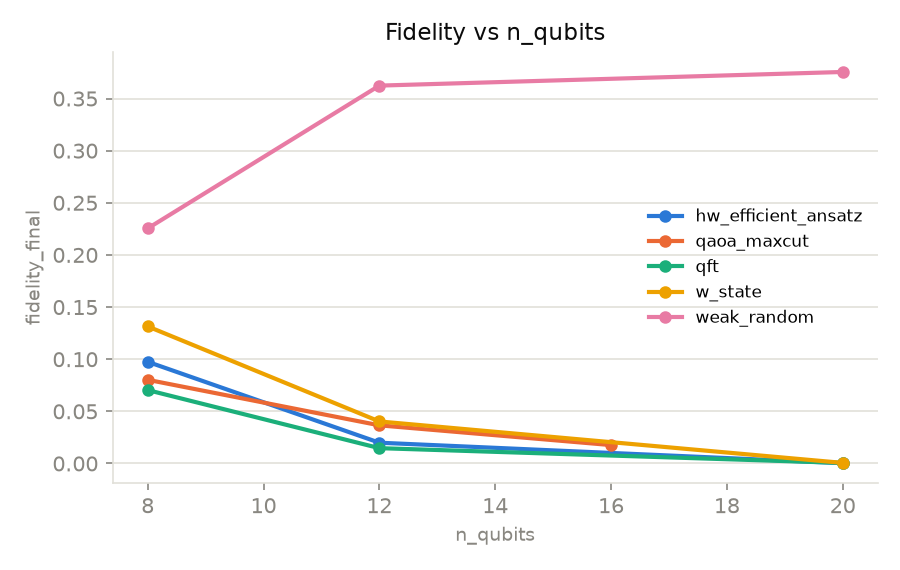
\includegraphics[width=0.75\linewidth]{figures/scaling_fidelity.png}
  \caption{Mean \texttt{fidelity\_final} vs.\ qubit count, per circuit
    family, pooled across the three per-block optimizers of the
    225-run core baseline (Section~\ref{sec:case-study:algorithms}).
    Four of five families decline toward the metric's near-zero floor
    as $n$ grows; \texttt{weak\_random} is the exception. A single-scale
    evaluation of any one family in isolation -- the norm in the
    QIEA-MOO literature surveyed above -- would surface only one point
    on this plot.}
  \label{fig:scaling-fidelity}
\end{figure}

More fundamentally, the
Pareto-dominance relation every classical MOEA baseline in
Section~\ref{sec:background:moea} and every NSGA-II-hybridized QIEA-MOO
method in Section~\ref{sec:taxonomy:hybridization} relies on has itself
only recently been shown to have a structural weakness --
\citet{zheng2025weakparetoboundary}'s ``weak Pareto boundary'' result --
that predates none of the surveyed QIEA-MOO literature's own
publication dates and so could not have been accounted for by any of
it. Scalability claims in this field, in short, rest on baselines and
dominance relations whose own limits are still being discovered, on top
of application-side evaluations that rarely test more than one problem
scale to begin with.
